\definecolor{myblue}{RGB}{166, 189, 219}
\definecolor{mygray}{RGB}{211, 211, 211}
\definecolor{mypink}{RGB}{255, 166, 201}
\definecolor{myred}{RGB}{255, 138, 138}
\definecolor{steelblue51132141}{RGB}{51,132,141}

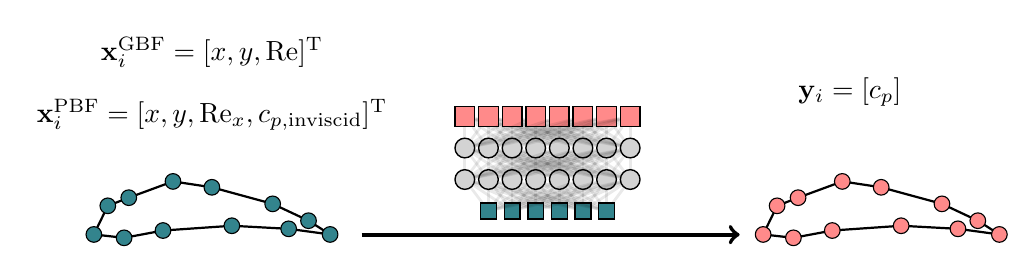
\begin{tikzpicture}[scale=1, 
                    nodeout/.style={rectangle, fill=myred, opacity=1, minimum width=2.5mm, minimum height=2.5mm, inner sep=0pt, line width=0.5pt, draw=black}, nodehidden/.style={circle, fill=mygray, opacity=1, minimum size=2.5mm, inner sep=0pt, line width=0.5pt, draw=black}, 
                    nodein/.style={rectangle, fill=steelblue51132141, minimum width=2mm, minimum height=2mm, inner sep=0pt, line width=0.5pt, draw=black}]

    \def\scaleFactor{3} % Define scaling factor
    \def\xShift{-1.5}

    % Define the points for the input airfoil shape with scaling
    \coordinate (P0) at ({\xShift + \scaleFactor * 0.9996}, {\scaleFactor * 0.0008});
    \coordinate (P1) at ({\xShift + \scaleFactor * 0.9083}, {\scaleFactor * 0.0590});
    \coordinate (P2) at ({\xShift + \scaleFactor * 0.7565}, {\scaleFactor * 0.1303});
    \coordinate (P3) at ({\xShift + \scaleFactor * 0.4992}, {\scaleFactor * 0.2004});
    \coordinate (P4) at ({\xShift + \scaleFactor * 0.3345}, {\scaleFactor * 0.2253});
    \coordinate (P5) at ({\xShift + \scaleFactor * 0.1474}, {\scaleFactor * 0.1564});
    \coordinate (P6) at ({\xShift + \scaleFactor * 0.0586}, {\scaleFactor * 0.1220});
    \coordinate (P7) at ({\xShift + \scaleFactor * -0.0004}, {\scaleFactor * 0.0008});
    \coordinate (P8) at ({\xShift + \scaleFactor * 0.1276}, {\scaleFactor * -0.0135});
    \coordinate (P9) at ({\xShift + \scaleFactor * 0.2922}, {\scaleFactor * 0.0174});
    \coordinate (P10) at ({\xShift + \scaleFactor * 0.5837}, {\scaleFactor * 0.0376});
    \coordinate (P11) at ({\xShift + \scaleFactor * 0.8242}, {\scaleFactor * 0.0246});
    \coordinate (P12) at ({\xShift + \scaleFactor * 0.9996}, {\scaleFactor * 0.0008});
    
    % Draw the airfoil shape
    \draw[thick] (P0) -- (P1) -- (P2) -- (P3) -- (P4) -- (P5) -- (P6) -- (P7) -- (P8) -- (P9) -- (P10) -- (P11) -- (P12) -- cycle;
    
    % Add circles at selected points
    \foreach \i in {1, 2, 3, 4, 5, 6, 7, 8, 9, 10, 11, 12} {
        \node[circle, draw, fill=steelblue51132141, inner sep=2pt] at (P\i) {};
    }
    
    % Define the points for the output airfoil shape
    % Define the shift in abscissa
    \def\xShift{7}

\coordinate (P0) at ({\xShift + \scaleFactor * 0.9996}, {\scaleFactor * 0.0008});
\coordinate (P1) at ({\xShift + \scaleFactor * 0.9083}, {\scaleFactor * 0.0590});
\coordinate (P2) at ({\xShift + \scaleFactor * 0.7565}, {\scaleFactor * 0.1303});
\coordinate (P3) at ({\xShift + \scaleFactor * 0.4992}, {\scaleFactor * 0.2004});
\coordinate (P4) at ({\xShift + \scaleFactor * 0.3345}, {\scaleFactor * 0.2253});
\coordinate (P5) at ({\xShift + \scaleFactor * 0.1474}, {\scaleFactor * 0.1564});
\coordinate (P6) at ({\xShift + \scaleFactor * 0.0586}, {\scaleFactor * 0.1220});
\coordinate (P7) at ({\xShift + \scaleFactor * -0.0004}, {\scaleFactor * 0.0008});
\coordinate (P8) at ({\xShift + \scaleFactor * 0.1276}, {\scaleFactor * -0.0135});
\coordinate (P9) at ({\xShift + \scaleFactor * 0.2922}, {\scaleFactor * 0.0174});
\coordinate (P10) at ({\xShift + \scaleFactor * 0.5837}, {\scaleFactor * 0.0376});
\coordinate (P11) at ({\xShift + \scaleFactor * 0.8242}, {\scaleFactor * 0.0246});
\coordinate (P12) at ({\xShift + \scaleFactor * 0.9996}, {\scaleFactor * 0.0008});
    % Draw the airfoil shape
    \draw[thick] (P0) -- (P1) -- (P2) -- (P3) -- (P4) -- (P5) -- (P6) -- (P7) -- (P8) -- (P9) -- (P10) -- (P11) -- (P12) -- cycle;
    
    % Add circles at selected points
    \foreach \i in {1, 2, 3, 4, 5, 6, 7, 8, 9, 10, 11, 12} {
        \node[circle, draw, fill=myred, inner sep=2pt] at (P\i) {};
    }


    % Draw thick arrow from input to output airfoil graph
    \draw[->, thick, black, line width=1.5pt] ({\scaleFactor * 1.1 - 1.4}, {\scaleFactor * 0.0}) -- ({\xShift - \scaleFactor*0.1 + \scaleFactor * 0.0}, {\scaleFactor * 0.0});


     % Draw MLP over the line
    % variables
    \def\deltax{0.3};
    \def\deltay{0.4};
    \def\mlpstartx{\scaleFactor * 1.17};
    \def\mlpstarty{\scaleFactor * 0.1};

        % Nodes
        % input
        % xi
        \node[nodein, fill=steelblue51132141, opacity=1] (ni1) at (\mlpstartx,\mlpstarty) {};
        \node[nodein, fill=steelblue51132141, opacity=1] (ni2) at (\mlpstartx+\deltax,\mlpstarty) {};
        \node[nodein, fill=steelblue51132141, opacity=1] (ni3) at (\mlpstartx+2*\deltax,\mlpstarty) {};

        % xj
        \node[nodein, opacity=1] (ni4) at (\mlpstartx+3*\deltax,\mlpstarty) {};
        \node[nodein, opacity=1] (ni5) at (\mlpstartx+4*\deltax,\mlpstarty) {};
        \node[nodein, opacity=1] (ni6) at (\mlpstartx+5*\deltax,\mlpstarty) {};

        % hidden layer 1
        \foreach \x in {1,...,8} {
            \pgfmathtruncatemacro{\layer}{1}
            \node[nodehidden] (nh\layer\x) at ({\mlpstartx+(\x-1)*\deltax-\deltax},{\mlpstarty+\layer*\deltay}) {};
            \foreach \prevnode in {1,...,6} {
                \draw[line width=1pt, color=mygray, opacity=0.085, draw=black] (ni\prevnode) -- (nh\layer\x);
            }
        }

        % hidden layer 2
        \foreach \x in {1,...,8} {
            \pgfmathtruncatemacro{\layer}{2}
            \node[nodehidden] (nh\layer\x) at ({\mlpstartx+(\x-1)*\deltax-\deltax},{\mlpstarty+\layer*\deltay}) {};
            \pgfmathtruncatemacro{\prevlayer}{\layer-1}
            \foreach \prevnode in {1,...,8} {
                \draw[line width=1pt, color=mygray, opacity=0.085, draw=black] (nh\prevlayer\prevnode) -- (nh\layer\x);
            }
        }

        % output
        \foreach \x in {1,...,8} {
            \pgfmathtruncatemacro{\layer}{3}
            \node[nodeout] (nh\layer\x) at ({\mlpstartx+(\x-1)*\deltax-\deltax},{\mlpstarty+\layer*\deltay}) {};
            \pgfmathtruncatemacro{\prevlayer}{\layer-1}
            \foreach \prevnode in {1,...,8} {
                \draw[line width=1pt, color=mygray, opacity=0.085, draw=black] (nh\prevlayer\prevnode) -- (nh\layer\x);
            }
        }
        
    
    % Add feature circle
    \coordinate (V_GBF) at ({\scaleFactor * 0.0}, {\scaleFactor * 0.0 + 2});
    % \filldraw[color=black, fill=myblue, thick](V_GBF) circle (0.1) node[] (V_GBF) {};
    \node at (V_GBF) [anchor=south] {$\mathbf{x}^{\mathrm{GBF}}_i = [x,y,\mathrm{Re}]^\mathrm{T}$};

    \coordinate (V_PBF) at ({\scaleFactor * 0.0}, {\scaleFactor * 0.0 + 1.2});
    % \filldraw[color=black, fill=myblue, thick](V_PBF) circle (0.1) node[] (V_PBF) {};
    \node at (V_PBF) [anchor=south] {$\mathbf{x}^{\mathrm{PBF}}_i = [x,y,\mathrm{Re}_x, c_{p, \mathrm{inviscid}}]^\mathrm{T}$};

    % % Add feature circle
    % \coordinate (V) at (-0.38,0.2);
    % \filldraw[color=black, fill=myblue, thick](-0.87,0.4) circle (0.08) node[] (n1) {$\mathbf{x}^{\mathrm{GBF}}_i = [x,y,\mathrm{Re}]^\mathrm{T}\mathbf{x}_i$};
    % \node at (V) [anchor=eastsouth] {$= [x,y,\mathrm{Re}]^\mathrm{T}\begin{bmatrix} x \\ y \\ \text{Re} \end{bmatrix}$};

    % \coordinate (V) at (-0.38,-0.4);
    % \filldraw[color=black, fill=mygreen, thick](-0.8,-0.1) circle (0.12) node[] (n1) {$\mathbf{x}^{\mathrm{PBF}}_i =[x,y,\mathrm{Re}_x, c_{p, \mathrm{inviscid}}]^\mathrm{T}\mathbf{x}^{\text{PBF}}_i$};
    % % \node at (V) [anchor=south] {$=[x,y,\mathrm{Re}_x, c_{p, \mathrm{inviscid}}]^\mathrm{T} \begin{bmatrix} x \\ y \\ \text{Re}_x \\ c_{p,\text{inviscid}}
    % \end{bmatrix}$};

    % Add prediction circle
    \coordinate (VO) at ({\xShift + \scaleFactor * 1.2 - 2.5}, 1.5);
    % \filldraw[color=black, fill=myred, thick](VO) circle (0.1) node[] (VO) {};
    \node at (VO) [anchor=south] {$\mathbf{y}_i =[c_p]$};


    \end{tikzpicture}